\chapter{Editor}
\label{cap:editor}

\section{Base del editor}

La base del desarrollo del editor se organiza en distintas secciones, clasificadas según su función principal dentro del sistema:

\begin{itemize}
	\item Elementos comunes: componentes comunes para todo el resto de componentes del editor, y que también permiten la comunicación entre estas distintas partes. Por ejemplo, la clase \texttt{Project}, que contiene toda la información referida a cada uno de los proyectos.
	\item Elementos de lectura-escritura: encargados de gestionar la entrada y salida de datos mediante archivos externos, permitiendo tanto la carga como el guardado de información.
	\item Elementos de dibujado: componentes encargados de la representación visual en pantalla. Aquí se incluyen todas las ventanas y \textit{subventanas} que componen la interfaz gráfica de la aplicación.
	\item Recursos: elementos del motor que pueden ser modificados desde el editor. Entre ellos, por ejemplo, mapas, objetos o \textit{sprites}.
\end{itemize}

\subsection{Elementos comunes}
Los elementos comunes son todos aquellos que no pertenecen exclusivamente a ninguna de las áreas especificadas (por ejemplo, gestión de la interfaz gráfica o gestión de recursos), sino que forman la base del funcionamiento del editor y su funcionalidad es compartida por múltiples partes del sistema.

\begin{itemize}
	\item \texttt{Editor}: implementado utilizando un patrón \textit{Singleton}, se encarga de crear y mantener una única instancia centralizada del editor. Su responsabilidad principal es inicializar todos los componentes esenciales (ventana principal, gestor de dibujado, gestor de entrada de usuario...) y coordinar su funcionamiento. Incorpora un método \texttt{mainLoop()} que ejecuta el bucle principal de la aplicación, el cual sigue una estructura típica de aplicaciones interactivas: captura de eventos de entrada del usuario, actualización del estado y dibujado de la interfaz. Gracias a esta arquitectura, se asegura una separación clara entre la lógica de control y la presentación visual.
	\item \texttt{Project}: representa la estructura y el contenido de cada proyecto creado con el editor. Esta clase centraliza la información relacionada con los recursos del proyecto, incluyendo mapas, \textit{sprites} u objetos. También, almacena las rutas relativas a los archivos en disco y proporciona métodos para modificar, cargar y guardar estos elementos. Además, ofrece una interfaz para la exportación o generación de la \textit{build} final del proyecto, asegurando así la persistencia y portabilidad del trabajo realizado por el usuario.
	\item \texttt{EditorError}: se encarga de gestionar los posibles errores, tanto de programación como de uso de la aplicación. Para ello, se utiliza la librería multiplataforma \texttt{tinyfiledialogs}, que permite mostrar alertas en pantalla de manera muy sencilla y sin inicialización previa.
\end{itemize}

En conjunto, estos elementos comunes proporcionan una infraestructura robusta y reutilizable sobre la que se construyen el resto de funcionalidades del editor, facilitando tanto su mantenimiento como su escalabilidad futura.

\subsection{Elementos de lectura-escritura}
Los elementos de lectura-escritura son todos aquellos componentes responsables de gestionar tanto la entrada del usuario como la lectura y escritura de datos del sistema, incluyendo preferencias, localización y proyectos.

\begin{itemize}
	\item \texttt{InputManager}: se encarga de inicializar y gestionar la entrada del usuario mediante teclado y ratón. Para ello, utiliza por debajo el método \texttt{SDL\_PollEvent()}, de la librería \texttt{SDL}, que permite obtener el último evento registrado en cualquiera de los periféricos del usuario\footnote{La implementación de SDL es esta, no puede haber dos eventos simultáneos y solo se registrará el último que se haya mandado. Por lo general, es complicado que haya dos eventos simultáneos, siempre hay una demora, por muy pequeña que sea, entre dos eventos.}. Este evento, posteriormente, es discriminado por el gestor dependiendo de si lo procesa la librería \texttt{DearImGui} mediante la llamada al método \texttt{ImGui\_ImplXXXX\_ProcessEvent()}\footnote{Se utiliza \texttt{XXXX} en medio del método ya que este es dependiente de la librería con la que se hubiese creado la ventana. En este caso, al estar creada utilizando \texttt{SDL3}, el método sería \texttt{ImGui\_ImplSDL3\_ProcessEvent()}.}, o si se procesa de manera independiente, por ejemplo, comprobando que el evento lanzado es el de cerrar la aplicación (\texttt{SDL\_EVENT\_QUIT}).
	\item \texttt{LuaManager}: se encarga de inicializar y gestionar la librería \texttt{sol3}, que permite interactuar mucho más amigablemente con Lua. Esta clase define métodos de serialización de tablas Lua utilizando un serializador externo, \texttt{serpent}, creado por Paul Kulchenko, que mantiene la legibilidad del archivo generado, facilitando tanto la depuración como la edición manual del mismo; un método que permite la escritura de una tabla Lua a un fichero \texttt{.lua}; y métodos para la creación de tablas Lua y lectura de tablas Lua desde un fichero de datos o un \textit{script}.
	\item \texttt{LocalizationManager}: se encarga de inicializar y gestionar la localización del proyecto, es decir, el idioma en el que aparecerá la interfaz. Para entender mejor la función de este gestor, se explicará el funcionamiento de los ficheros de idiomas del editor.
	\begin{itemize}
		\item El editor cuenta con ficheros \texttt{.lua}, nombrados siguiendo la especificación IETF BCP 47 \citep{rfc5646}\footnote{Esta especificación define un idioma de la siguiente manera: \comillas{id\_PA}, donde \textit{id} es una abreviación del idioma y \textit{PA} una abreviación del país donde se habla ese idioma. Por ejemplo, para el español de España, su código BCP 47 sería \comillas{es\_ES}, y para el inglés estadounidense, \comillas{en\_US}.}, que contienen una tabla de Lua cuya clave es un identificador definido para un determinado texto en el editor, y el valor es la frase requerida en el idioma correspondiente. Por ejemplo:
\begin{figure}[t]
 \begin{minipage}{0.48\textwidth}
  \centering
  \begin{minted}[fontsize=\footnotesize]{lua}
return {
  ["action.settings"] = "Ajustes",
  ["action.add"] = "Añadir",
  ["window.mapeditor"] = "Mapa"
}
  \end{minted}
  \caption{\small Contenido del fichero\\ \texttt{es\_ES.lua}.}
  \label{fig:luaes}
 \end{minipage}
 \hfill
 \begin{minipage}{0.48\textwidth}
  \centering
  \begin{minted}[fontsize=\footnotesize]{lua}
return {
  ["action.settings"] = "Settings",
  ["action.add"] = "Add",
  ["window.mapeditor"] = "Map"
}
  \end{minted}
  \caption{\small Contenido del fichero\\ \texttt{en\_EN.lua}.}
  \label{fig:luaen}
 \end{minipage}
  \label{fig:lualang}
\end{figure}

	En la tabla Lua de la figura \ref{fig:luaes} se observa la traducción en español, y en la tabla de la figura \ref{fig:luaen}, la traducción en inglés. Ambos ficheros comparten las mismas claves, por ejemplo, \texttt{action.settings}, que se referirá al texto que aparece en un botón que lleve hacia la pantalla de configuración del editor.
	\item El gestor de localización obtendrá la \textit{locale}\footnote{Las \textit{locales} o configuraciones regionales son todos los parámetros, definidos en el sistema operativo de un ordenador, que definen el idioma, país y preferencias especiales que el usuario quiera ver en su interfaz (por ejemplo, el formato de la fecha y hora o la divisa).} preferida del usuario, utilizando el método \texttt{SDL\_GetPreferredLocales()}, e intentará cargar el archivo \texttt{.lua} cuyo nombre sea el de la \texttt{locale} preferida que haya devuelto el método. Si no se encuentra un archivo con el mismo identificador BCP 47, se intentará cargar el fichero con el mismo idioma\footnote{Por ejemplo, una persona argentina tendrá configurado su ordenador de tal manera que la \textit{locale} será \comillas{es\_AR}. Al no haber un fichero \texttt{es\_AR.lua}, cargará uno que tenga el mismo idioma, es decir, \texttt{es\_ES.lua}.}, y si el idioma tampoco se encuentra, cargará por defecto el idioma inglés.
	\item Una vez cargado el fichero, se guardará el contenido en un diccionario clave-valor, y se podrá acceder a cualquier frase requerida utilizando la clave guardada en el fichero Lua. Por ejemplo, si se quisiese, desde código, obtener la frase detrás de \texttt{action.add}, bastará con llamar a \texttt{getString(``action.add")}.
	\item También está contemplado el cambio de idioma por parte del usuario, por lo que el gestor también cuenta con un método, \texttt{changePreferredLocale()} que permite el cambio de idioma del editor sin más complejidad.
	\item Este sistema es bastante ampliable, ya que simplemente para añadir un nuevo idioma, basta con crear un fichero \texttt{.lua} cuyo nombre sea el identificador BCP 47 del idioma correspondiente, copiar todas claves de uno de los ficheros existentes, y posteriormente generar la traducción. Este tipo de ampliaciones se suele hacer utilizando plataformas como \textit{Crowdin} (\url{https://crowdin.com/}), que permiten traducciones hechas por individuos de manera altruista en múltiples idiomas.
	\end{itemize}
	\item \texttt{PreferencesManager}: gestiona las preferencias del usuario en cuanto al editor. El sistema está preparado para leer y guardar las preferencias del usuario desde un archivo \texttt{userPreferences.lua}, almacenado junto al ejecutable del editor, y poder utilizarlas durante el código, haciendo una llamada al método \texttt{getPreference()} con el identificador de la preferencia. El proyecto, de momento, solo almacena la preferencia de idioma del usuario, pero está implementado de manera que puede ser escalable a cualquier preferencia nueva que se quiera añadir. Las preferencias se guardan automáticamente cuando se modfican por parte del usuario, por lo que no es necesario tener que hacer un guardado manual de estas.
	\item \texttt{ProjectManager}: gestiona todos los proyectos creados por el usuario en su ordenador. \texttt{ProjectManager} se encarga de leer el fichero \texttt{projects.lua}, que contiene todas las rutas de todos los proyectos y almacenar instancias de la clase \texttt{Project} sin inicializar\footnote{Si se inicializase la instancia de \texttt{Project} en el momento de la lectura, y, el usuario tuviese creados muchos proyectos, sería un gran gasto de memoria innecesario, por lo que la instancia solo se inicializa en el momento en el que el editor va a necesitar poder obtener sus datos y modificarlos.}. Posteriormente, se comprueba que la ruta guardada por el editor en el fichero \texttt{projects.lua} existe y en ella se encuentra un archivo \texttt{ProjectSettings.lua}. En el caso de que este fichero no exista o tenga un formato incorrecto, el gestor ignora dicha entrada y la interfaz del editor se encargará de mostrar una advertencia al usuario. El gestor permite también eliminar proyectos, crear nuevos, añadir otros ya existentes y reubicar aquellos en los que no se encuentre un fichero \texttt{ProjectSettings.lua} válido.
\end{itemize}

Cabe destacar, que todos estos gestores están implementados utilizando un patrón \textit{singleton}, por lo que una única instancia es válida para todas las clases del proyecto y no es necesario tener que estar gestionando el paso de punteros entre las distintas clases.

\medskip

En conjunto, estos gestores permiten que el editor funcione de manera modular y adaptable a las necesidades del usuario, facilitando tanto la personalización como la persistencia de datos y configuraciones entre sesiones.

\subsection{Elementos de dibujado}
\label{subsec:dibujado}
Los elementos de dibujado son los responsables del dibujado en pantalla de la interfaz del editor. Estas clases están diseñadas para trabajar conjuntamente con la librería \texttt{DearImGui} y el motor de renderizado de \texttt{SDL3}, facilitando la gestión de la interfaz gráfica y el contenido visual del entorno de desarrollo.

\begin{itemize}
	\item \texttt{RenderObject}: es una interfaz que implementan todos los objetos que dibujan algo en pantalla. Define el método \texttt{render()}, que las clases que implementen esta interfaz tienen que redefinir.
	\item \texttt{WindowStack}: es una pila de objetos \texttt{RenderObject} a \textit{renderizar} de abajo a arriba\footnote{Esto, que puede parecer contradictorio ya que en principio rompería el propósito de una pila, cuya función es solo tener acceso al elemento más superior de esta. El diseño de esta pila está pensado para, gestionar el añadir y quitar ventanas como una pila tradicional, pero poder recorrerla para su renderizado de abajo a arriba.}, es decir, se dibujará primero el elemento que esté en la parte inferior de la pila, y sucesivamente hasta el superior. Esta clase contiene métodos para añadir y eliminar objetos de \textit{render}, y un método, \texttt{renderWindows()} para poder recorrer todos estos elementos en orden y llamar a su método \texttt{render()}.
	\item \texttt{RenderManager}: se encarga de gestionar todo el apartado gráfico del editor, y, como el resto de gestores, está implementado utilizando un patrón \textit{singleton}. Inicializa la ventana de la aplicación, así como el aparado gráfico de \texttt{SDL} y \texttt{DearImGui}, y tiene métodos para el manejo y obtención de parámetros de la ventana principal de la aplicación, métodos que permiten la carga de un fichero \texttt{.ttf} de fuentes vectoriales o que permiten la carga de texturas e imágenes. Por otra parte, cuenta con el método \texttt{render()}, llamado desde el bucle principal del editor, y que gestiona el ciclo de dibujado de la aplicación, llamando a la función \texttt{renderWindows()} de \texttt{WindowStack} y posteriormente vuelca en la pantalla del usuario todo el contenido de \textit{render} actualizado desde la última llamada. 
	\item \texttt{Window}: es una interfaz que implementan todas las ventanas principales de la aplicación. Esta interfaz, que hereda de \texttt{RenderObject}, implementa el método \texttt{render()} de la siguiente forma:
\begin{center}
	\begin{minipage}{0.6\textwidth}
		\begin{minted}{c}
void Window::render() {
	beforeRender();
	ImGui::Begin();
	onRender();
	ImGui::End();
}
		\end{minted}
	\end{minipage}
\end{center}
	De esta manera, cada ventana que se quiera generar implementando esta interfaz solo tiene que redefinir los métodos \texttt{beforeRender()}, que se usa principalmente para modificar atributos asociados a \texttt{DearImGui}; y el método \texttt{onRender()}, que contiene el dibujado propiamente dicho del contenido de la ventana.
	\item \texttt{Subwindow}: se denomina \comillas{subventana} a todos aquellos elementos que componen una ventana (es decir, una ventana está compuesta por subventanas). Estas \comillas{subventanas} son un \textit{wrapper}\footnote{Es decir, un envoltorio o estructura que encapsula una funcionalidad para simplificar su funcionamiento y uso.} de las clases \texttt{Child} pertenecientes a la librería \texttt{DearImGui}. La implementación de esta clase es idéntica a la de la clase \texttt{Window}, sustituyendo las llamadas a \texttt{ImGui::Begin()} por \texttt{ImGui::BeginChild()}.
	\item \texttt{ModalWindow}: una ventana modal es una ventana o caja de diálogos que aparece en la interfaz y que bloquea la interacción con el resto de la aplicación hasta que el usuario la cierra o responde. Este tipo de ventanas se utiliza para acciones críticas o que requieran de atención inmediata, por ejemplo, asistentes de creación de elementos (\textit{wizards}). \texttt{DearImGui} permite el uso de modales utilizando las clases \texttt{Popup} y \texttt{PopupModal}; sin embargo, este uso tiene una limitación, y es que solo un modal puede estar activo en un determinado momento, y para poder lanzar otro es necesario cerrarlo. Sin embargo, esta limitación no ha entorpecido el desarrollo del proyecto, y se ha podido desarrollar toda la funcionalidad sin problema ninguno.
	\item \texttt{WindowItem}: esta clase es un \textit{wrapper} de la clase \texttt{TabItem} de \texttt{DearImGui}, que representa una pestaña dentro de una barra de pestañas (\texttt{TabBar}). Esta clase permite organizar el contenido en secciones separadas dentro de una misma ventana, sin la necesidad de tener que gestionarlo mediante \comillas{subventanas} y con la posibilidad del cambio entre pestañas sin abrir nuevas ventanas.
\end{itemize}

En conjunto, estos elementos permiten una arquitectura modular y extensible para la construcción de la interfaz gráfica del editor, facilitando tanto el mantenimiento del código como la integración de nuevas funcionalidades visuales de forma ordenada y eficiente.

\subsection{Recursos}
Los recursos permiten representar en el editor todos aquellos elementos que posteriormente serán utilizados por el motor del juego para su funcionamiento.

\begin{itemize}
	\item \texttt{EditorResource}: es la interfaz común que deben implementar todos los recursos. Estos tienen que tener, necesariamente, sobrescritas e implementadas las siguientes tres funciones:
	\begin{itemize}
		\item \texttt{readFromLua()}: lee los datos desde un fichero \texttt{.lua} de uno de los recursos utilizando llamadas a métodos de \texttt{LuaManager}.
		\item \texttt{writeToLua()}: implementa la escritura de uno de los recursos a un fichero \texttt{.lua} para su guardado en disco, también utilizando llamadas a métodos de \texttt{LuaManager}.
		\item \texttt{writeToEngineLua()}: implementa la \comillas{traducción} de uno de los recursos del editor a la sintaxis esperada por los recursos del motor, escribiéndolo también en un fichero \texttt{.lua}.
	\end{itemize}
	\item \texttt{Sprite}: define un \textit{sprite}, es decir, una imagen bidimensional que representa un objeto o un personaje en pantalla. De los \textit{sprites} se guarda su textura (generada utilizando el \texttt{RenderManager}) y las dimensiones de esta, así como métodos que permiten su obtención y modificación.
	\item \texttt{Animation}: define una animación, es decir, una lista de \texttt{Sprite} que actúan como fotogramas y que se suceden rápidamente para representar movimiento o cambios visuales de un objeto. De las animaciones se guarda una lista de \texttt{Sprite}, el tiempo entre fotogramas (fijado en el proyecto de 0.01s hasta 5s) y si la animación se repite en bucle. 
	\item \texttt{Tile}: representa una baldosa, es decir, la unidad básica para construir los mapas en el editor. La baldosa es una imagen de dimensiones fijas (en el caso de este Proyecto, mínimo de 8x8 píxeles y máximo de 256x256), y las baldosas se generan a partir de un \texttt{Tileset}, por lo que simplemente se almacena su textura y su índice dentro del \textit{tileset}.
	\item \texttt{Tileset}: representa una colección de objetos \texttt{Tile} organizados en una sola imagen (habitualmente en forma de cuadrícula). Es decir, en el caso del editor, un \texttt{Tileset} es una lista de \texttt{Tile}, ordenados de izquierda a derecha y de arriba a abajo. Para ahorrar trabajo a la hora de establecer las colisiones en el mapa a los usuarios, cada una de las \textit{tiles} tiene asociada un \textit{booleano} indicando si se puede colisionar o no con ese tipo de baldosa en concreto.
	\item \texttt{Event}: los eventos, explicados en el apartado \ref{sec:eventos}, permiten agregar lógica a un juego sin la necesidad de programar. Cada evento tiene asociado uno o varios comportamientos y una única condición de ejecución. Estos comportamientos y condiciones corresponden a las clases \texttt{EventBehaviour} y \texttt{EventCondition}. Las condiciones se ejecutan en orden, de arriba a abajo, por lo que la clase \texttt{Event} permite el cambio de orden de ejecución de las condiciones. Tanto los eventos como las condiciones se crean utilizando el \comillas{patrón factoría}, por lo que también se disponen de las clases \texttt{EventBehaviourFactory} y \texttt{EventConditionFactory}, que en su método \texttt{Create()} devuelven bien un comportamiento o una condición solamente con el identificador de cada uno de ellos. A continuación, se explican brevemente cada uno de los comportamientos:
	\begin{itemize}
		\item \texttt{AnimationBehaviour}: permite reproducir, detener, reiniciar y cambiar una animación.
		\item \texttt{ChoicesBehaviour}: permite generar, en un diálogo, tres opciones como máximo a escoger y cambiar el valor a una variable dependiendo de la opción elegida.
		\item \texttt{DialogueBehaviour}: permite mostrar un texto en pantalla.
		\item \texttt{JumpBehaviour}: permite hacer un salto a otros comportamientos, parecido a la instrucción \texttt{goto} en algunos lenguajes de programación.
		\item \texttt{JumpIfBehaviour}: permite hacer un salto a otros comportamientos si se cumple una determinada condición, es decir, es un salto condicional.
		\item \texttt{ModifyVariableBehaviour}: permite cambiar el valor de una variable, bien sea de un objeto o de un jugador.
		\item \texttt{MoveBehaviour}: permite mover un objeto un determinado número de casillas, tanto en horizontal como en vertical.
		\item \texttt{MusicBehaviour}: permite reproducir, detener, reanudar, pausar, cambiar audio, cambiar volumen y establecer si una pista de sonido está o no en bucle.
		\item \texttt{PlaySFXBehaviour}: permite reproducir un efecto de sonido.
		\item \texttt{WaitForBehaviour}: hace una espera hasta que se cumpla una determinada condición.
	\end{itemize}
	Y, a continuación, se explican brevemente cada una de las condiciones:
	\begin{itemize}
		\item \texttt{AlwaysCondition}: esta condición siempre se cumple. Equivale al \texttt{true} en los lenguajes de programación.
		\item \texttt{AndCondition}: esta condición permite concatenar otras dos condiciones, y se cumplirá siempre y cuando las dos condiciones que concatene se cumplan.
		\item \texttt{BehaviourEndedCondition}: esta condición se cumple cuando un comportamiento termine.
		\item \texttt{CollidesWithPlayerCondition}: esta condición se cumple cuando un objeto colisione con el jugador.
		\item \texttt{InteractionCondition}: esta condición se cumple cuando se interactúe con un objeto.
		\item \texttt{NotCondition}: niega todas las condiciones, por lo que se cumplirá siempre y cuando la condición que niegue no se cumpla.
		\item \texttt{OnStartCondition}: esta condición se cumple al inicio de un evento.
		\item \texttt{OrCondition}: esta condición también permite concatenar otras dos condiciones, y se cumplirá siempre y cuando al menos una de las dos condiciones que concatene se cumpla.
		\item \texttt{TimePassedCondition}: esta condición se cumple cuando haya transcurrido un determinado tiempo.
		\item \texttt{ValueEqualsCondition}: esta condición se cumple cuando el valor de una variable equivalga a un determinado valor.
	\end{itemize}
	\item \texttt{Object}: define un objeto de juego. Esta clase añade métodos para establecer la posición del objeto en el mapa, establecer la capa del mapa en la que se encuentra, añadir o eliminar variables y eventos, y establecer su \texttt{Sprite}.
	\item \texttt{Map}: define un mapa. Los mapas tienen un máximo de 16 capas, y están compuestos por elementos de la clase \texttt{Tile}. Los mapas, a su vez, tienen colisiones en cada una de las casillas de la cuadrícula y también pueden albergar un objeto por cada una de ellas.
\end{itemize}

Estas clases constituyen la base del sistema de edición de datos del proyecto, proporcionando estructuras reutilizables y extensibles que permiten almacenar, modificar y traducir los datos del editor al formato legible del motor, facilitando la interacción entre el editor y el entorno de ejecución.

\section{Interfaz del editor}
En cuanto a la interfaz que compone el editor, toda ella está elaborada utilizando la librería \texttt{DearImGui} junto con todos los elementos de dibujado mencionados en el apartado \ref{subsec:dibujado}. 

\begin{figure}[t]
	\centering
	%
	\begin{SubFloat}
		{\label{fig:welcomewindow}%
		Ventana de bienvenida de \baker.}%
		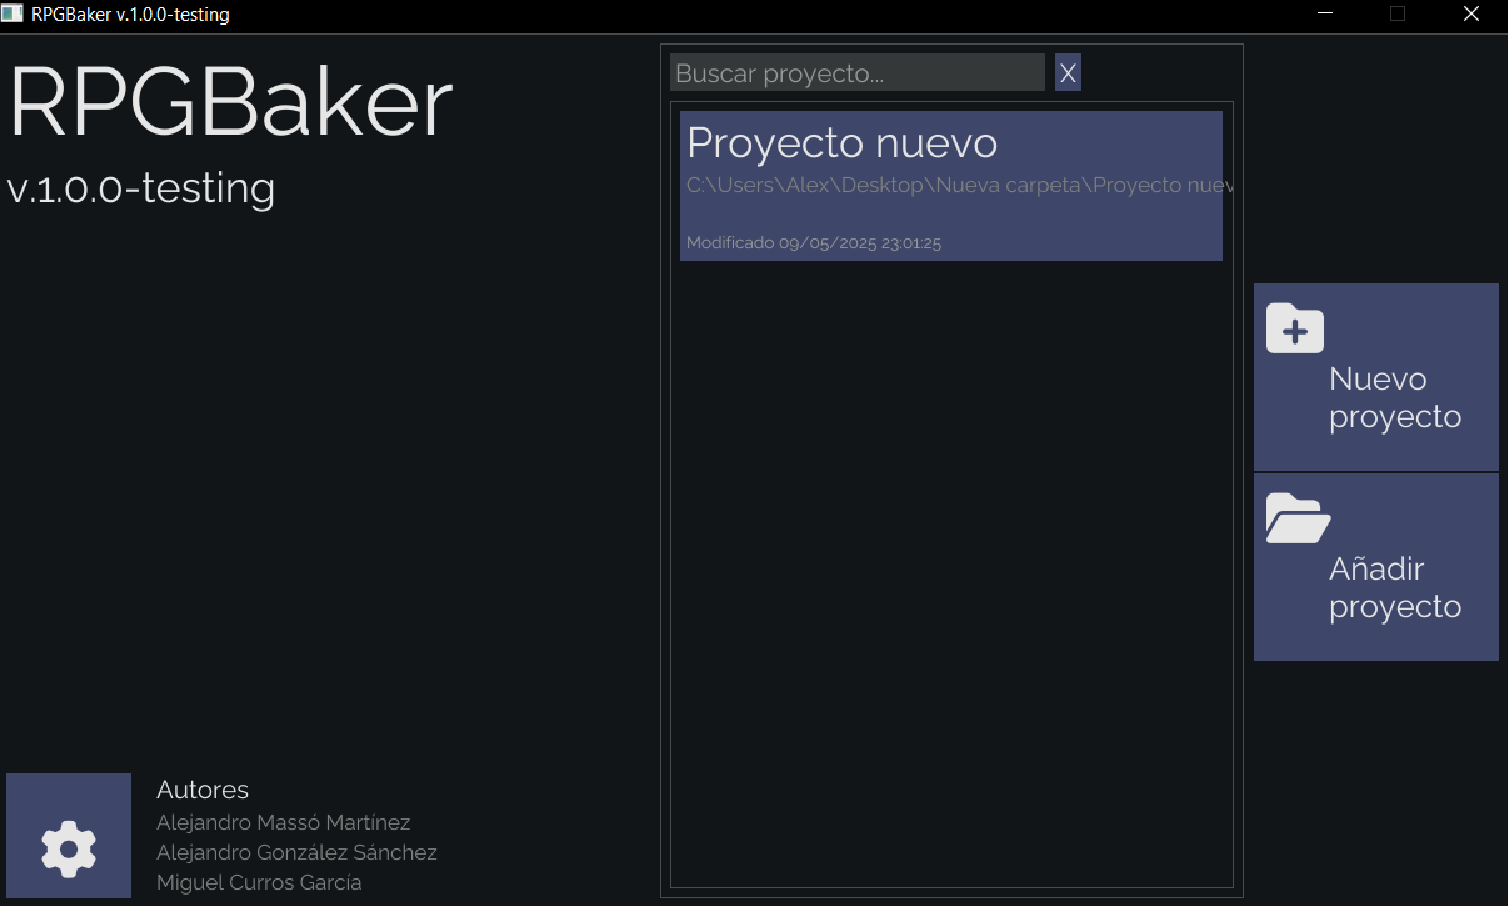
\includegraphics[width=0.45\textwidth]{Imagenes/Vectorial/welcomewindow}%
	\end{SubFloat}
	\qquad
	\begin{SubFloat}
		{\label{fig:eventwindow}%
		Ventana de edición de eventos de \baker.}%
		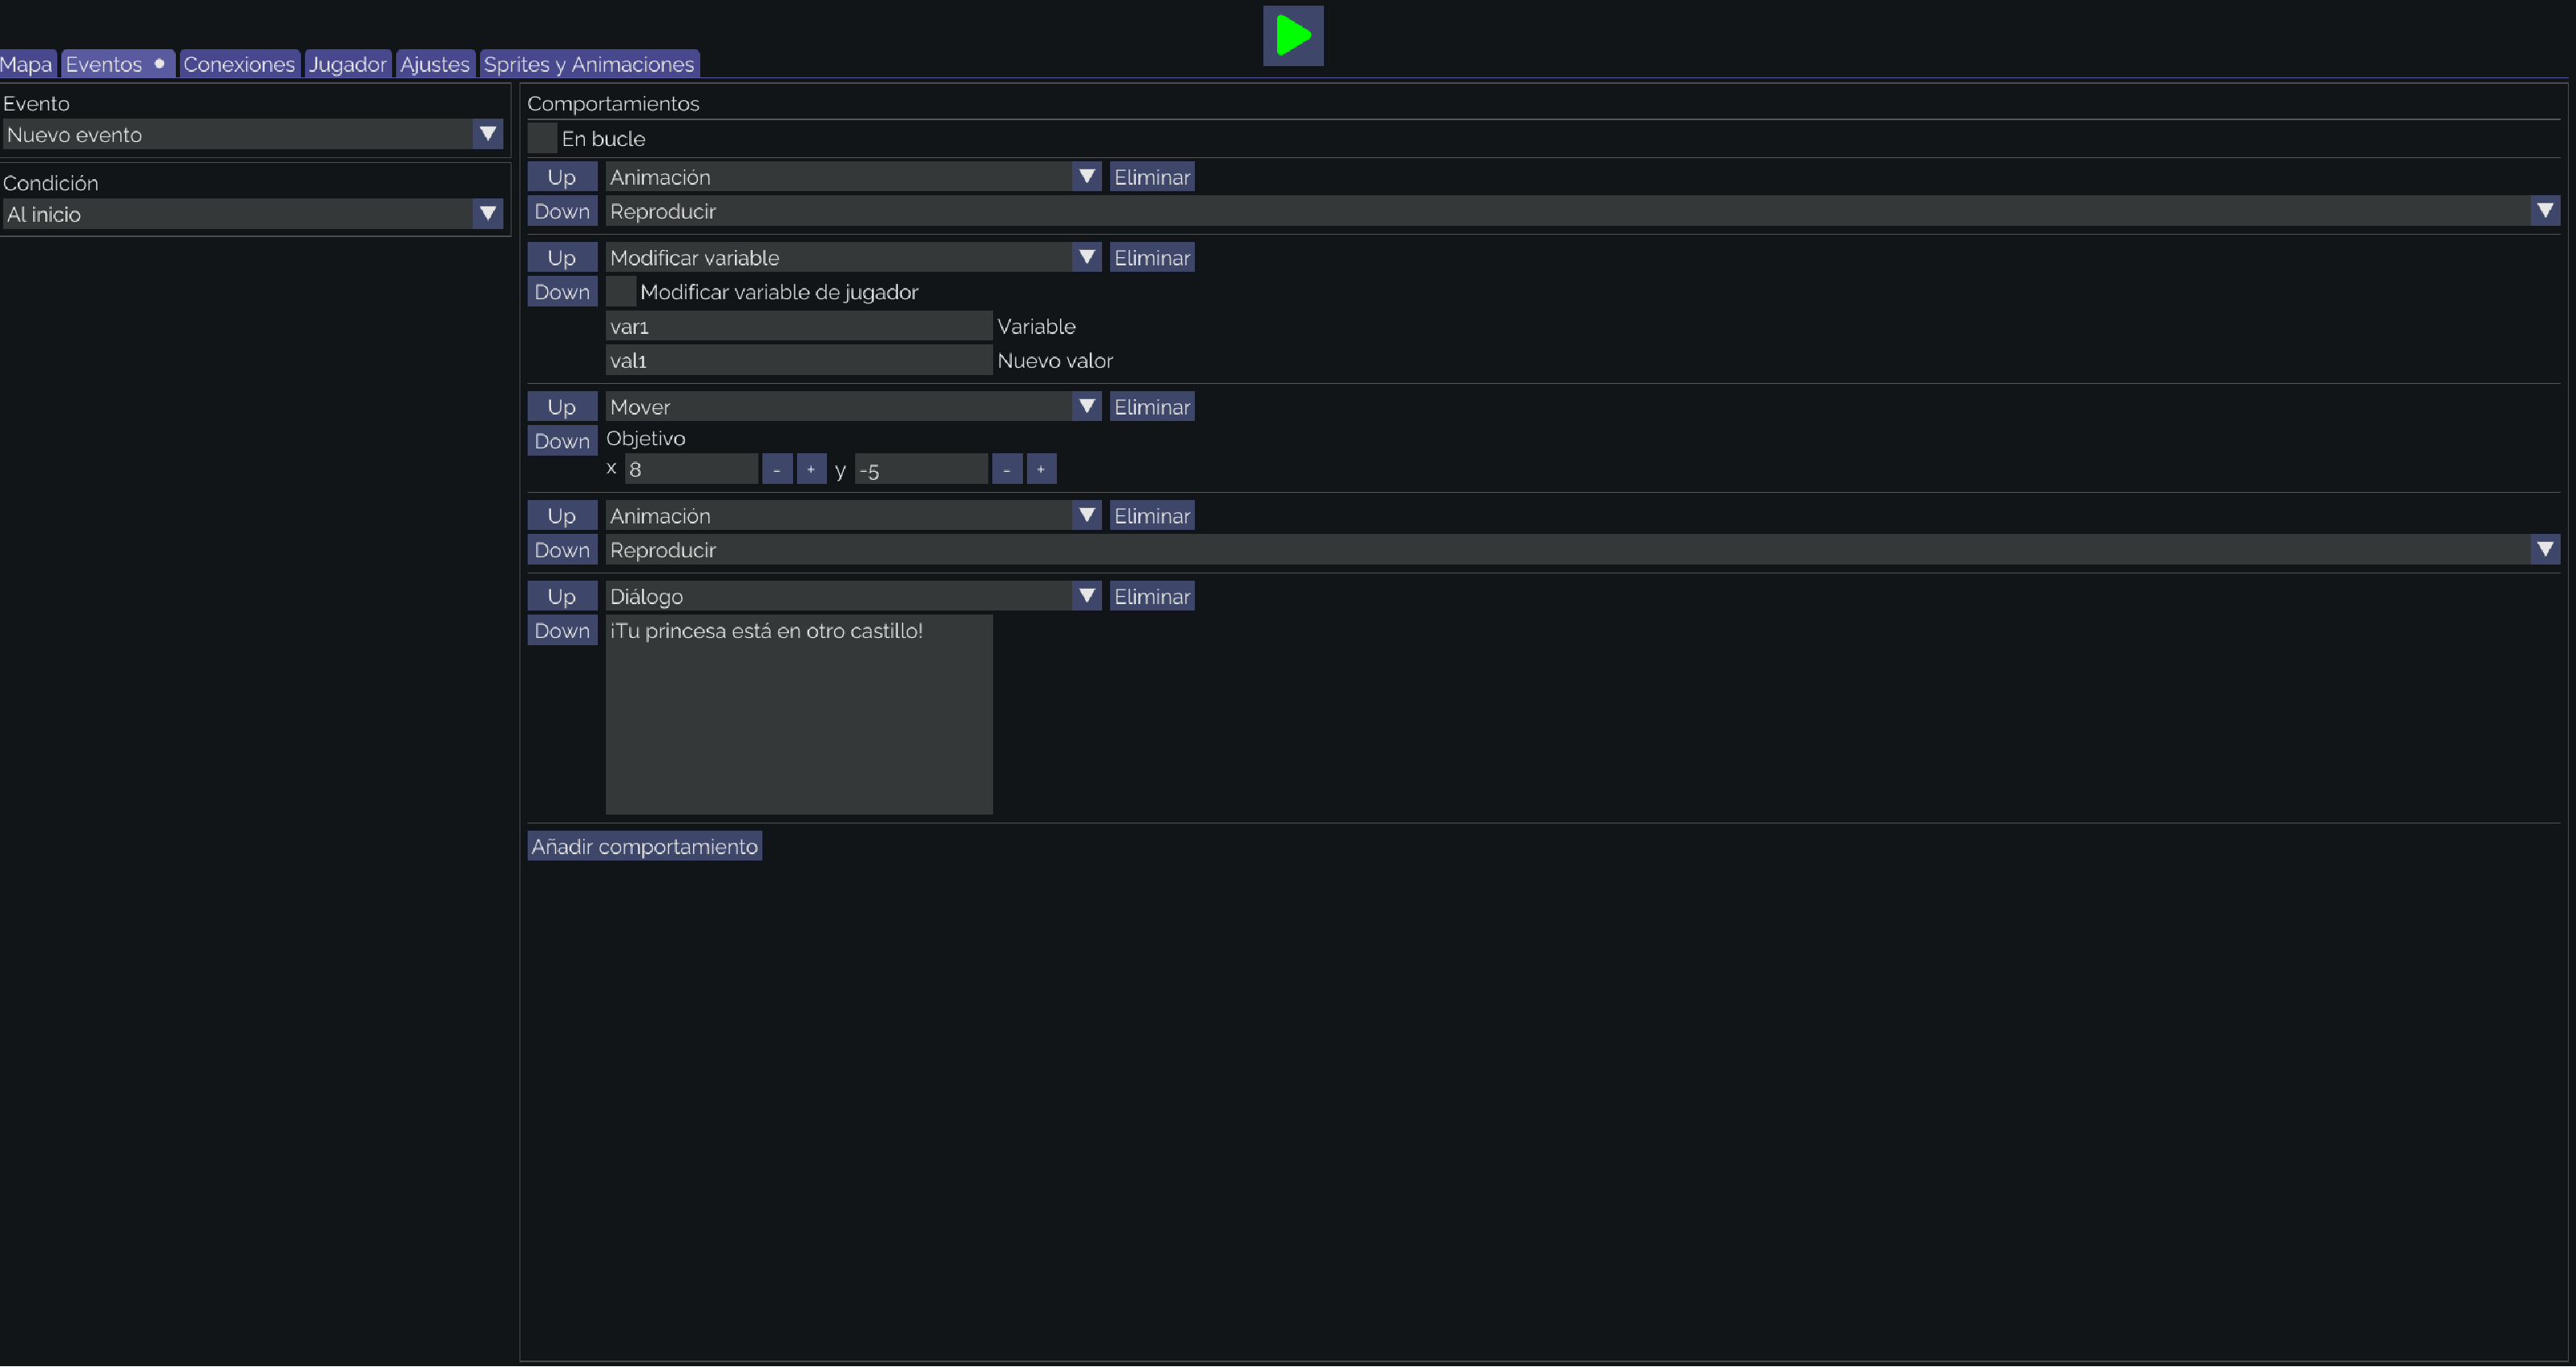
\includegraphics[width=0.45\textwidth]{Imagenes/Vectorial/eventos}%
	\end{SubFloat}
	%
	\begin{SubFloat}
		{\label{fig:conexiones}%
		Ventana de conexiones entre mapas de \baker.}%
		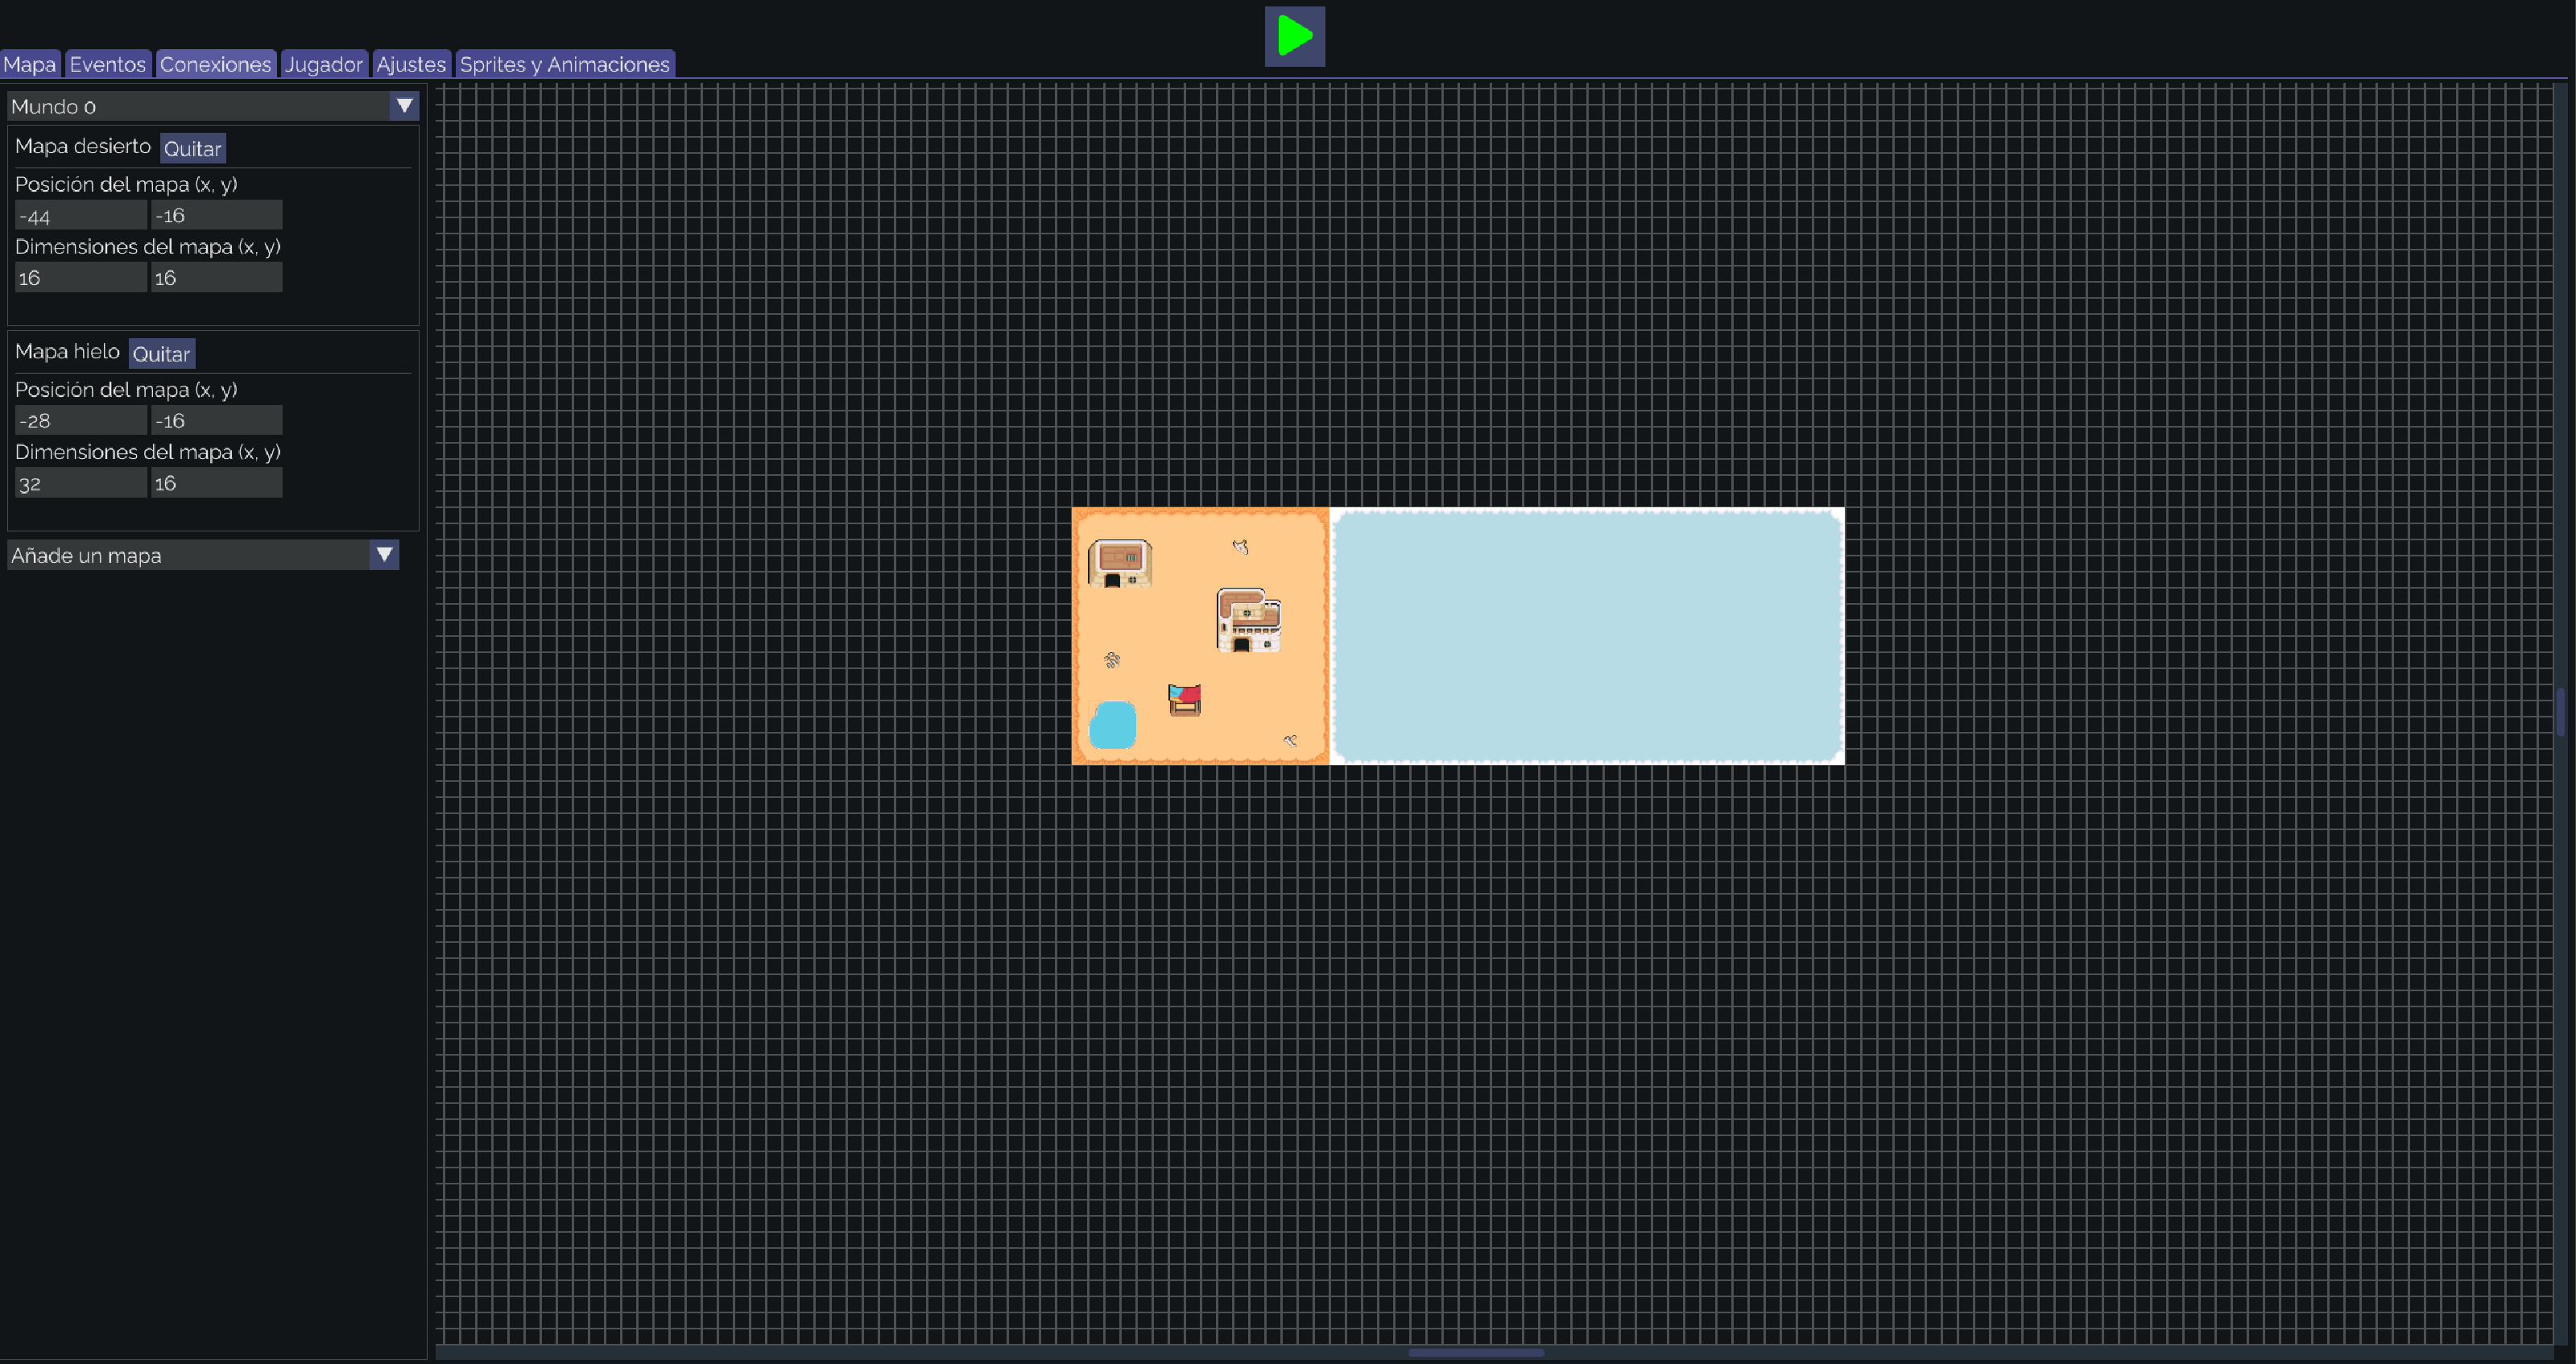
\includegraphics[width=0.45\textwidth]{Imagenes/Vectorial/conexiones}%
	\end{SubFloat}
	\qquad
	\begin{SubFloat}
		{\label{fig:playerwindow}%
		Ventana de edición del jugador de \baker.}%
		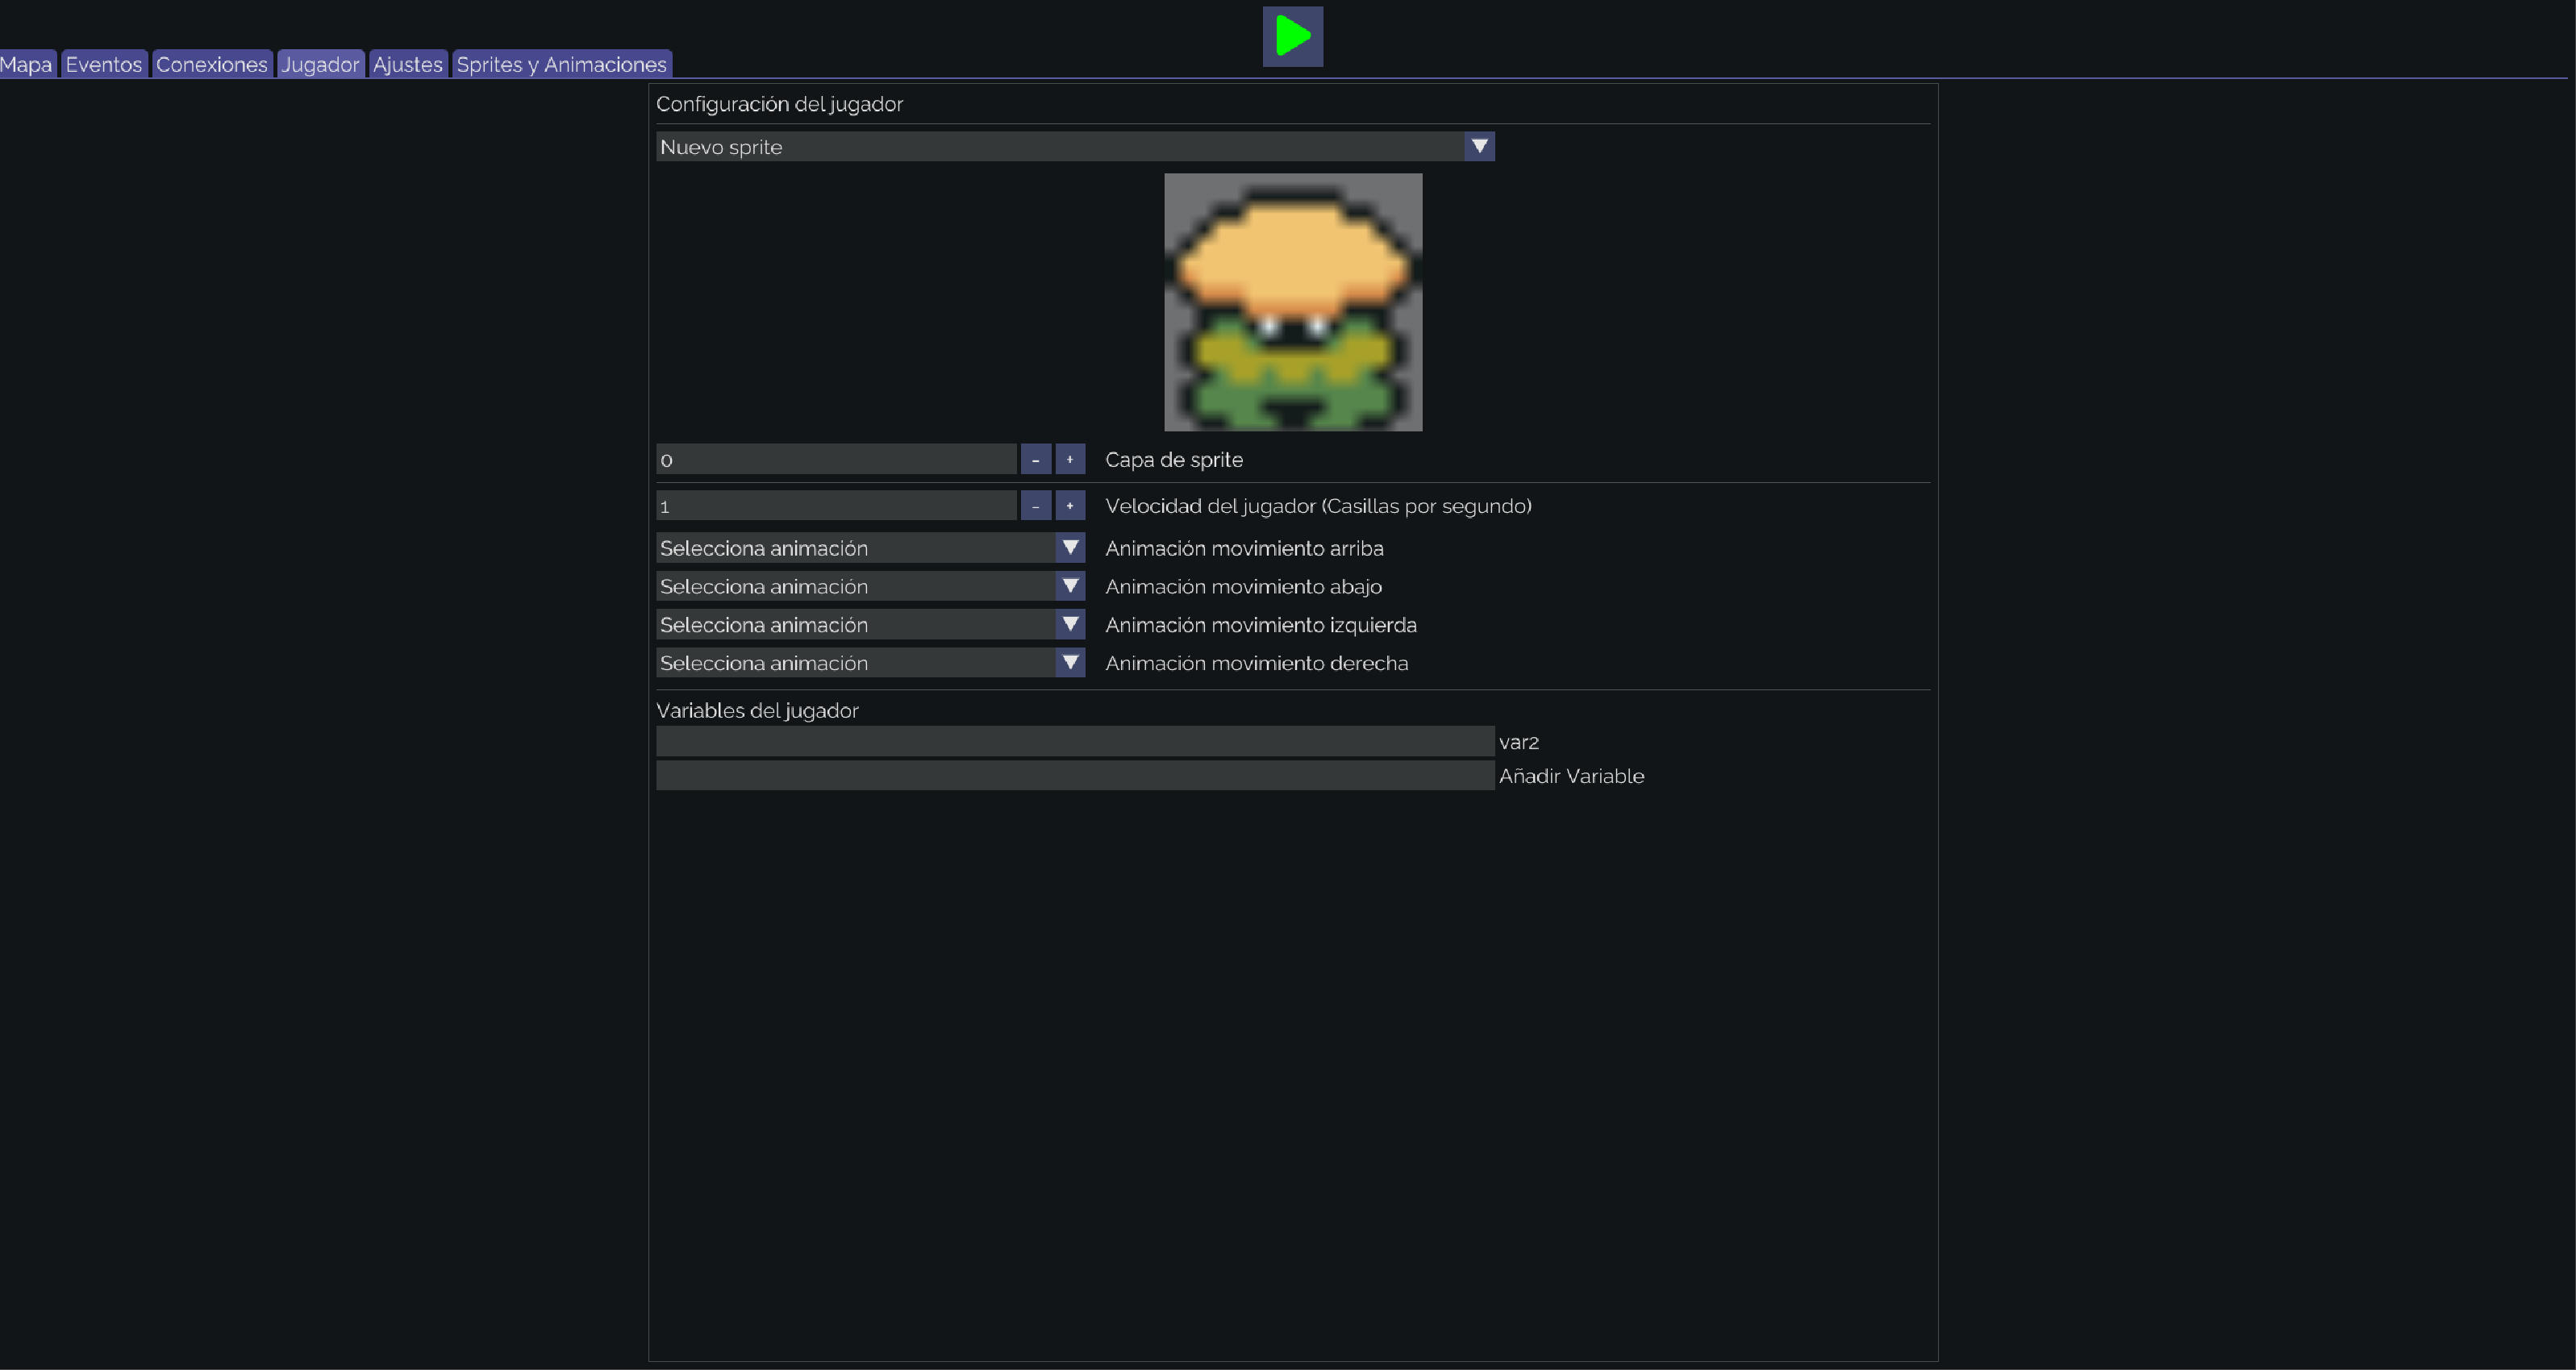
\includegraphics[width=0.45\textwidth]{Imagenes/Vectorial/jugador}%
	\end{SubFloat}
	\caption{Distintas ventanas del editor de \baker. \label{fig:menusbaker}}
\end{figure}

\begin{itemize}
	\item La ventana de bienvenida (figura \ref{fig:welcomewindow}), que permite la gestión de todos los proyectos creados por el usuario, así como crear uno nuevo y añadir otro ya existente, y también cambiar el idioma de la interfaz.
	\item La ventana principal de la aplicación, que permite la edición de un proyecto en concreto y está dividida en varias pestañas, cada una con una función distinta:
	\begin{itemize}
		\item El editor de mapas (figura \ref{fig:mapeditor}), permite la creación y modificación de un mapa utilizando diversos \textit{tilesets}. En la parte izquierda se encuentra el visor de \textit{tilesets}, que permite crear nuevas a partir de un fichero de imagen, editar las ya presentes o eliminarlas. En la parte central se encuentra el editor \textit{per se}, mostrándose una cuadrícula con el tamaño elegido por el usuario. Esta cuadrícula se puede ampliar y alejar, y tiene varios modos de visualización:
		\begin{itemize}
			\item Visualización de la capa actual exclusivamente.
			\item Visualización de la capa actual y las de abajo con transparencia.
			\item Visualización de la capa actual y las de abajo completamente opacas.
			\item Visualización de todas las capas en conjunto, empezando desde abajo hasta arriba.
		\end{itemize}
		Finalmente, en la parte derecha, se encuentra el editor de objetos, que permite crear y eliminar un objeto y agregarle o eliminarle un \textit{sprite}, un evento o una variable.
		\item El editor de eventos (figura \ref{fig:eventwindow}), que permite la creación y edición de eventos, añadiendo los comportamientos esperados y las condiciones de lanzamiento. Eventos complejos se encapsulan dentro de otros y todos se pueden ordenar por orden de prioridad de ejecución utilizando las flechas que aparecen al costado izquierdo.
		\item El editor de conexiones (figura \ref{fig:conexiones}), que permite crear mundos\footnote{Un mundo, en la jerarquía de nuestro Proyecto, es aquel elemento que puede contener diversos mapas.} y añadirle los mapas, modificando en la cuadrícula la posición final de cada uno de los mapas.
		\item El editor del jugador (figura \ref{fig:playerwindow}), que permite establecer ajustes del jugador, como por ejemplo su \textit{sprite}, sus animaciones de movimiento en las cuatro direcciones cardinales básicas y variables propias de este.
		\item El editor de ajustes, que permite editar información relevante al ejecutable final, como por ejemplo, el nombre de la ventana, las dimensiones que la cámara puede mostrar en pantalla de una sola vez, el mapa en el que empezará el jugador o la fuente por defecto que mostrarán los textos.
		\item El editor de \textit{sprites} y animaciones, que permite generar un \textit{sprite} a partir de un \textit{spritesheet} o de una imagen, estableciendo el \textit{offset} que se desee, y, posteriormente, a partir de los \textit{sprites}, poder generar una animación. El asistente de creación de animaciones contiene un visor en tiempo real de la animación, así como controles para poder navegar por los diversos fotogramas.
	\end{itemize}
\end{itemize}